\section{Ziel}
In diesem Versuch wird die Funktionsweise eines Geiger-Müller-Zählrohrs betrachtet.
Es werden die Kennlinien der Betriebsspannung und die Totzeit der gegebenen Apparatur ermittelt.

\section[Theorie]{Theorie\footnote[1]{Unter Verwendung von \cite{man:v703}.}}
Geiger-Müller-Zählrohre gibt es in verschiedenen Versionen.
Die meisten haben aber einen Metallzylinder einen Zählrohrdraht meist aus Wolfram. 
Der Zylinder ist mit einer dünnen Mylarfolie oder einem Glimmer verschlossen, welche gleichzeitig als
Eintrittsfenster dienen.
In der Kammer eingeschlossen ist ein Edelgas, welches mit Kohlenwasserstoffen versetzt ist.
Zwischen dem Draht un dem Zylinder ist eine Spannung angelegt.

Tritt ionisierende Strahlung in die Kammer ein, wird das Gasgemisch im Innern der Kammer ionisiert.
Durch die Angelegte Spannung werden die Ionen von zum Draht oder zum Zylinder hin beschleunigt.
Auf dem Weg dahin können die Elektronen bzw. Ionen bei einer ausreichenden Spannung weitere Gasmoleküle ionisieren, sodass eine Kettenreaktion ausgelöst wird.
Das führt wiederum zu einer großen Anzahl an Ladungsträgern, die über einen Widerstand abfließen.
Da der Widerstand im Megaohmbereich liegt führt dieser Prozess zu einem Abfall in der Spannung, der die Kettenreaktion dann unterbricht.
Mit einem Verstärker kann dieser kurzzeitige Spannungsabfall in einem Zählgerät oder einem Oszilloskop gemessen werden.
Die Zeit dieses Spannungsabfalls wird auch Totzeit genannt, da keine weiteren Strahlungen während dieser Zeit gemessen werden können.


\begin{figure}
    \centering
    \input{14_v703/Inhalte/A_Test.pdf_tex}
    \caption{Die Zählrohrcharakteristik.}
    \label{fig:02_teo}
\end{figure}

Die Zählrate des Geiger-Müller-Zählrohrs hängt von der Betriebsspannung ab.
Diese Abhängigkeit wird Zählrohrcharakteristik genannt. 
Folgende Bereiche sind dabei relevant
\begin{itemize}
    \item \textbf{Rekombination:} Bei einer niedrigen Betriebsspannung werden keine Zerfälle gemessen.
    Die gebildeten Ionen können sich auf dem Weg zum Anodendraht wieder mit Elektronen zu neutralen Atomen verbinden.
    \item \textbf{Ionisationskammer:} Ab einer gewissen Spannung erreichen alle Elektronen bzw Ionen die Elektroden, und es wird ein Sättigungsstrom erreicht.
    In diesem Bereich kommen nur die Elektroden und Ionen an, die direkt von der Strahlung erzeugt werden.
    \item \textbf{Proportionalitätsbereich:} Wenn die Spannung weiter erhöht wird, können die Elektronen mit Stoßionisation weitere Elektronen Ionen Paare erzeugen. 
    Dieser Prozess passiert in der Nähe des Anodendrahts sehr häufig was zu einer Verstärkung des Spannungsabfalls um einen Faktor der Größenordnung \num{1e3} führt.
    % Die Verstärkung ist hierbei abhängig von der Art der Strahlung
    \item \textbf{Geiger-Müller-Bereich:}
    Hier können alle Arten von radioaktiver Strahlung gleichgut detektiert werden.
    Im gesamten Zählrohr bilden sich Townsend-Lawinen, wobei die Elektronen über den Anodendraht abfließen.
    Die trägeren Ionen bilden eine Raumladungswolke, die weitere Lawinen behindert. 
    So entstehen Impulse gleicher Höhe unabhängig von der Art oder Energie der einfallenden Strahlung.
    In diesem Spannungsbereich können die Gasatome in einen Angeregten Zustand versetzt werden.
    In diesem Zustand können sie Photonen aussenden, die mit dem Photoeffekt Elektronen von der Wand lösen können.
    Diese können weitere Townsend-Lawinen erzeugen, die ein Störfaktor in der Messung sind.
    Die Photonen können mit einem Löschgas, dem Alkohol absorbiert werden.
    \item \textbf{Dauerentladung:} Eine weitere Erhöhung der Spannung Führt zu einer Dauerentladung, die Das Zählrohr zerstören kann. 
\end{itemize}

Das Zählratenplateau hat bei realistischen Geiger-Müller-Zählrohren eine Steigung $s$.
Diese hängt damit zusammen, dass Strahlung, die die Ränder des Messzylinders Sekundärelektronen auslösen kann, die Zeitversetzt weitere Impulse lostreten.
Dieser Effekt wird vermieden, indem ein Löschgas aus Langkettigen Alkohol-Molekülen die Kinetische Energie dieser Elektronen aufnimmt.
Die Wahrscheinlichkeit, dass das nicht funktioniert hängt von der angelegten Spannung und dem Alter des Geiger-Müller-Zählrohres ab.
Die Steigung $s$ ist also ein Maß für die Qualität des Zählrohres
\begin{align}
    s = \frac{\Delta n}{n} \cdot \qty{100}{\percent}/\qty{100}{\volt}
\end{align}
Sie ist Bezogen auf die relativen Zählraten pro \qty{100}{\volt} definiert.

\noindent
Wenn ein Impuls in dem Geiger-Müller-Bereich verstärkt wird bildet sich ein Ionengas um den Anodendraht.
Dieses verhindert dass in dieser Zeit weitere Strahlung gemessen werden kann.
Die Zeit in der keine Strahlung gemessen werden kann heißt Totzeit.
Wenn die Ladungen abgegeben wurden können die Impulse erst nicht mit voller Intensität auftreten bis sich die Ionen ausgeglichen haben.
Diese Phase nennt sich Erholungsphase. 
Das dazugehörige Oszilloskop-bild ist in Abbildung \ref{fig:03_teo} zu sehen.
\begin{figure}
    \centering
    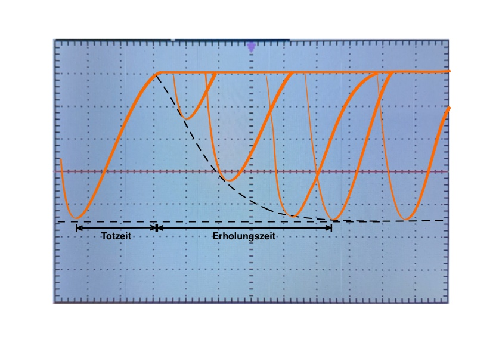
\includegraphics[width = 0.75\textwidth]{14_v703/Abbildungen/tod.pdf}
    \caption{Tot- und Erholungszeit auf einem Oszilloskopbild}
    \label{fig:03_teo}
\end{figure}

Bei der Zwei-Quellen Methode wird die Totzeit ermittelt, indem man davon ausgeht, dass bei einer größeren Anzahl an Zerfällen mehr Zerfälle nicht gemessen werden. 
Im Vergleich von den Zählraten zweier Proben $N_1$ und $N_2$ mit der Zählrate für beide Proben zusammen $N_{12}$ ergibt sich die folgende Formel für die Totzeit $\tau$
\begin{align}
    \tau = \frac{N_1 + N_2 - N_{12}}{N_{12}^2 -N_{1}^2 - N_{2}^2 }.
    \label{eq:zwei_quellen}
\end{align}


\section{Vorbereitung}
In diesem Versuch wird eine \ce{^{204}Tl}-Quelle verwendet.
Laut der Nuklidkarte \cite{nuklidkarte} zerfällt \ce{^{204}Tl} in einem $\beta^{-}$ Zerfall zu \ce{^{204}Pb} und in einem $\beta^{+}$ Zerfall zu \ce{^{204}Hg}. 
Die Halbwertszeit beträgt \num{3.783} Jahre.
Die Unsicherheit bei der Zerfallsrate $n$ beträgt
\begin{align}
    \Delta n &= \sqrt{n} & \frac{\Delta n}{n} = \frac{\sqrt{n}}{n} \leq 0.01
\end{align}
da die Zerfallsrate eine poissonverteilte Größe ist.
Es ergibt sich  eine Zerfallsrate vom $n \geq \qty{10000}{1\per\second}$ um einen Fehler von \qty{1}{\percent} zu erreichen.